%-------------------------------------------------------------------------------
% seq66 sessions
%-------------------------------------------------------------------------------
%
% \file        sessions.tex
% \library     Documents
% \author      Chris Ahlstrom
% \date        2020-10-03
% \update      2021-12-05
% \version     $Revision$
% \license     $XPC_GPL_LICENSE$
%
%  Provides a discussion of how Seq66 supports session management, specifically
%  the Non Session Manager.
%
%-------------------------------------------------------------------------------

\section{Session Management}
\label{sec:sessions}

   Session management helps recreate complex setups and provide some uniformity
   of application control.
   The first thing to do for session management is to make sure that the
   application is capable of various levels of session management, from
   \textsl{UNIX} signals to
   a complete session manager like the \textsl{Non Session Manager}.
   Basic session management consist of being able to properly start the
   application and let it run properly during its life-cyle, whether it is a
   command-line application or a graphical application.
   \textsl{Seq66} supports session management in three ways:

   \begin{enumber}
      \item \textbf{Signals}.
         During a normal run, \textsl{Seq66} will respond
         to signals to save and to quit.
         The normal configuration files and command-line options will be used.
         This mode is useful with \textsl{nsm-proxy}, a way to script
         applications that don't have \textsl{NSM} support.
      \item \textbf{JACK Session}
         Deprecated, but implemented nonetheless.
         This allows for the configuration files to be stored in
         a separate directory, for \textsl{Seq66} to be started, and files to be
         saved.  No restrictions on where the MIDI files can be stored.
      \item \textbf{Non Session Manager}
         Known as NSM, it provides a replacement for \textsl{JACK Session}.
         It requires all files to be
         stored in a session directory, and provides commands for saving,
         quitting, hiding/showing the user-interface, and more.
         Like \textsl{JACK Session}, it allows control over the startup of
         multiple applications, the process of saving a session, and provides a
         way to save their patching (connections) in \textsl{JACK}.
         However, it supports more functionality and has
         strict requirements the application must follow.
         Development of NSM has, for various reasons, been suspended, but
         offshoots such as \textsl{Agordejo} (\cite{agordejo}
         and \textsl{RaySession} (\cite{raysession})
         continue to advance.
   \end{enumber}

   If one desires session management, \textsl{NSM} is the way to go.
   \textsl{JACK} session management is provided for those who still use it.
   There are other session solutions, such as \textsl{aj-snapshot},
   \textsl{Claudia}, and \textsl{Chino}.
   For now, we do not discuss them.

   The desired session can be set in the \textbf{Edit / Preferences /
   Session} tab.  But note that, if started by \textsl{NSM}, \textsl{Seq66}
   will still set up for NSM usage.  The \textsl{NSM} setting is
   useful for attaching to a pre-existing known session.
   Also, \textsl{JACK} session management event are only processed
   if \textsl{JACK} is selected.
   \textsl{JACK} session management will still start \textsl{Seq66} in
   an existing session, if \textsl{JACK} is
   not selected, but that's it.

   Also note that sometimes one will want the session manager to make the JACK
   connections.  In this case, go to
   \textbf{Edit / Preferences / JACK / Jack Auto-Connect}, uncheck that option,
   and restart \textsl{Seq66}.  This option (\texttt{jack-auto-connect}
   can also be changed in the 'rc' file.

\subsection{Session Management / Signals}
\label{subsec:sessions_signals}

   \index{sessions!signals}
   By default, the basic form of session management in
   \textsl{Seq66} occurs by signals.  A
   session manager can start \textsl{Seq66}, and it can tell \textsl{Seq66} to
   save or stop.  Starting is done by a system call to spawn the application.
   The save and stop actions are supported by sending the following signals to
   the application:

   \begin{itemize}
      \item \texttt{SIGINT}.
         This signal stops \textsl{Seq66}. It corresponds
         to using \texttt{Ctrl-C} from the command-line to stop \textsl{Seq66}.
         This signal should work for both the graphical and command-line
         application.  As \textsl{Seq66} shuts down, it does its normal saving
         of the current state of the configuration.
      \item \texttt{SIGTERM}.
         This signal also stops \textsl{Seq66}.  It can
         be sent by an application to exit \textsl{Seq66}.
      \item \texttt{SIGUSR1}.
         This signal tells \textsl{Seq66} to save.  This
         action will save the current MIDI file.
   \end{itemize}

   One application that can control \textsl{Seq66}, to some extent, when not in
   session mode, is \textsl{nsm-proxy}:

      \url{https://non.tuxfamily.org/wiki/nsm-proxy}

   \textsl{NSM-Proxy} is a simple \textsl{NSM} client for wrapping non-NSM
   capable programs. It enables the use of programs supporting LADISH Level 0
   and 1, and programs which accept their configuration via command-line
   arguments.  There is a command-line version and a graphical version.

   More to come on how to use \texttt{nsm-proxy}.

\subsection{Session Management / JACK Session}
\label{subsec:sessions_jack}

   Although deprecated by the \textsl{JACK} authors in favor of \textsl{NSM},
   we are implementing \textsl{JACK} session (JS) management for the benefit of
   people who either do not know of \textsl{NSM} or do not want to implement or
   use it.

   \textsl{Seq66}, as a JS-aware applications, is set up to

   \begin{enumerate}
      \item Register with a JS manager.
      \item Respond to messages from the JS manager.
      \item Be startable with session information.
   \end{enumerate}

   A response to a JS message will do one of the following:

   \begin{itemize}
      \item Save the application's state into a file, where the directory is
         supplied by the session manager.
      \item Reply to the session manager with a command-line that starts the
         application, with information to restore its state, such as
         the name of the file holding its state information.
   \end{itemize}

	JS-aware clients identify themselves to the session manager by a UUID
	(unique universal identifier). The session manager provides it to
	the client application as an integer represented as a string.
   This can be passed to the session manager when registering, but
   \textsl{Seq66} just uses the value given to it (for now).

%  but should also be passed back to the client when it is restarted
%by the session manager. This is done by a command line argument to the
%application, and the format of the command line is also up to the client.

   For this discussion, we will use the \textsl{JACK} session implementation in
   the \textsl{QjackCtl} application.
   Also, read the script stored in
   \texttt{seq66/data/linux/startqjack} to set up
   \textsl{QjackCtl} to run \textsl{JACK} and kick off
   \textsl{a2jmidid}; it should be added to the \textsl{QjackCtl}
   configuration.

   Once that setup is made (installing the script and configuring
   \texttt{qjackctl}, then start \texttt{qjackctl}.
   Verify that there are a number of system audio and MIDI playback and capture
   port, \textsl{PulseAudio JACK} sinks and sources if the system uses
   \textsl{PulseAudio}, and that there are "a2j" MIDI ports for all of your USB
   hardware devices.

   Then start \textsl{Qsynth} so it uses \textsl{jack} for MIDI and
   \textsl{jack} (or \textsl{pulseaudio}) for audio.

   Then run \textsl{Seq66} with \textsl{JACK} for slave transport and for MIDI:

   \begin{verbatim}
      $ qseq66 --jack-slave --jack-midi
   \end{verbatim}

   Load a file, make sure its MIDI output goes to "fluidsynth" or "qsynth", and
   plays.

   In your desired location (e.g. \texttt{~/.config/seq66/sessions},
   create a new session directory (e.g. \texttt{qtest}).

   In \textsl{qjackctl}, open the \textbf{Sessions} dialog.
   Click \textbf{Save}, and choose the directory just created.
   In the dialog should appear entries for MIDI capture and playback for
   "fluidsynth" and "seq66", all the "a2j" USB devices,
   plus an entry for \textsl{JACK} client
   \textsl{seq66master} or \textsl{seq66slave} that shows
   something like:

   \begin{verbatim}
qseq66 --jack-midi --jack-master --jack-session-uuid 84670 --home ${SESSION_DIR}
qseq66 --jack-midi --jack-slave --jack-session-uuid 84670 --home ${SESSION_DIR}
   \end{verbatim}

   In the \textbf{Connections} dialog of \textsl{QjackCtl}, all of these ports
   will be shown in the MIDI tab, auto-connected appropriately.
   In the sessions directory that was created, will be seen an
   empty \texttt{seq66master}
   or \texttt{seq66slave} directory, and a
   \texttt{sessions.xml} configuration file containing the information shown in
   the sessions dialog.

   Exit \textsl{Seq66}, \textsl{QSynth} and \textsl{QjackCtl}
   (in that order).

   One issue is that \textsl{QSynth}
   does not support \textsl{JACK Session}.
   Try it with \textsl{Yoshimi}, which does support it.

% /usr/local/bin/qseq66 --jack-session-uuid 8589934670 --home
% /home/ahlstrom/Home/ca/mls/git/seq66/sessions/qsynth-test-2/seq66_transport/

\subsection{Seq66 Session Management / NSM}
\label{subsec:sessions_nsm}

   \index{sessions!nsm}
   The \textsl{Non Session Manager} is an API implementation for session
   management for Linux audio/MIDI. NSM clients use a well-defined
   \index{sessions!OSC}
   \textsl{OSC} protocol to communicate with the session management daemon.

   Note that \textsl{Non Session Manager} is in a state of suspended
   development, and has been reimplemented as a \textsl{GitHub} project,
   the \textsl{New Session Manager}.

   The applications it manages should be installed normally (that is,
   for system-wide usage, in
   \texttt{/usr/bin/} or \texttt{/usr/local/bin}).

\subsubsection{Session Management / NSM / First Run Without NSM}
\label{subsec:sessions_nsm_first_run_without_nsm}

   This section discusses what happen when \textsl{Seq66} is installed, then
   run outside of any session from the console or an application menu.
   For a discussion where \textsl{Seq66} is run for the first time under
   \textsl{NSM},
   see \sectionref{subsec:sessions_nsm_first_run_in_nsm}.

   Generally, after installing \textsl{Seq66}, or when creating a new setup
   (such as a play-list) it is good to run it normally first, to simplify
   trouble-shooting.
   This action creates the configuration files in the default location,
   \texttt{/home/user/.config/seq66}:

\begin{verbatim}
   $ qseq66 
   No 'rc' file, will create: qseq66.rc/ctrl/midi/mutes
   No 'usr' file, will create: /home/user/.config/seq66/qseq66.usr
   File exists: /home/user/.config/seq66/qseq66.rc
   Saving initial config files to session directory!
   Writing 'rc': /home/user/.config/seq66/qseq66.rc
   Writing 'ctrl': /home/user/.config/seq66/qseq66.ctrl
   Writing 'mutes': /home/user/.config/seq66/qseq66.mutes
   Writing 'usr': /home/user/.config/seq66/qseq66.usr
   . . .
\end{verbatim}

   Then exit \textsl{Seq66} to ensure the configuration files are created.
   Optionally, in this initial setup,
   one can also create a 'playlist' file and a 'drums' file, or
   copy them from:

   \begin{verbatim}
      /usr/share/seq66-0.91/data/samples
   \end{verbatim}

   to

   \begin{verbatim}
      /home/user/.config/seq66
   \end{verbatim}

   and modify them appropriately.
   Another first-time modification to consider is setting up \textsl{Seq66} to
   use the \textsl{JACK} audio/MIDI subsystem (on \textsl{Linux}).
   In the 'rc' file, look for the following line:

   \begin{verbatim}
      [jack-transport]
      jack-midi = false
   \end{verbatim}

   And change it to:

   \begin{verbatim}
      [jack-transport]
      jack-midi = true
   \end{verbatim}

   Another first-time modification to consider is using virtual ports (option
   \texttt{--manual-ports}) versus the automatic port connections
   \textsl{Seq66} normally makes.
   This setup allows the user to manually make connections between
   \textsl{Seq66} and other MIDI applications.
   In the 'rc' file, look for the following lines:

\begin{verbatim}
   [manual-ports]
   virtual-ports = false   # 'true' = manual (virtual) ALSA or JACK ports
   output-port-count = 8   # number of manual/virtual output ports
   input-port-count = 4    # number of manual/virtual input ports
\end{verbatim}

   And change the virtual-ports line to:

\begin{verbatim}
   [manual-ports]
   virtual-ports = true    # 'true' = manual (virtual) ALSA or JACK ports
\end{verbatim}

   It is then important to start \texttt{qseq66} in the normal manner again,
   and verify that everything works as expected.

   \textbf{Warning}.
   As the next section shows, if one wants to start with a
   \textsl{blank} NSM configuration,
   simply \textsl{move or hide}
   any existing \textsl{Seq66} configuration files from the
   "HOME" (\texttt{/home/user/.config/seq66})
   configuration directory before
   creating an NSM session and adding \textsl{Seq66} to it.

   We are considered expanding the \textbf{File / Import into session...}
   command to do this automatic importing manually.
   \index{NSM!template}
   On the other hand, the user can use the configuration
   in \texttt{/home/user/.config/seqq66} as a stock configuration
   to use as a \textsl{template} when creating a new session.

\subsubsection{Seq66 Session Management / NSM / Run in NSM}
\label{subsec:sessions_nsm_first_run_in_nsm}

   When \textsl{Seq66} is run in \textsl{NSM} for the first time,
   what happens to the new configuration depends on whether or not 
   the normal configuration files exist in the normal (no session)
   default configuration location.

   If \textsl{no} configuration files exist,
   then new configuration files are created
   in the \textsl{NSM} session directory.
   If these configuration files \textsl{do} exist,
   then they are \textsl{replicated} in the \textsl{NSM} session directory.
   If the configuration specifies play-lists, the whole play-list, including
   the MIDI files, are replicated in the NSM session.

   \textbf{No existing normal configuration}.
   Here, we have just installed \textsl{Seq66}, but have not
   yet run it.  We start the \textsl{non-session-manager}, create a new session,
   and add \texttt{qseq66} to this session.  This starts \texttt{qseq66}, and,
   after a short delay to get the session information from the daemon, a new
   configuration is created in the session directory.

   \textbf{Existing normal configuration}.
   If there is an existing \textsl{Seq66} configuration,
   then running \texttt{qseq66} in a new
   session will cause the normal configuration to be recreated in the new
   session directory, including play-lists and MIDI files.
   If a play-list has been configured, it is also
   copied, and so are the MIDI files it requires. (Their relative directory
   structure is preserved.)

   If \textsl{JACK} has been configured to be
   used by \textsl{Seq66}, be sure \textsl{JACK} is started (e.g. by running
   the \textsl{qjackctl} application.)

   For illustration, we run \textsl{NSM} from a terminal window, which can be
   very helpful when problems occur.

\begin{verbatim}
   $ non-session-manager
   [non-session-manager] Starting daemon...
   [nsmd] Session root is: /home/user/NSM Sessions
   NSM_URL=osc.udp://mycomputer.mls:19625/
   [nsmd] Listing sessions
\end{verbatim}

   \index{sessions!non-starter}
   If \textsl{NSM} refuses to start, make sure that the \texttt{liblo} library
   from the OSC project is installed.  If it is installed, then check the
   \texttt{/etc/hosts} file to make sure that the loopback interfaces are
   defined. In some versions of \textsl{Linux}, it isn't defined properly,
   and the \textsl{NSM} daemon (\texttt{nsmd}) will not start.
   Here is an example for the default install in \textsl{Debian Sid};

\begin{verbatim}
   127.0.0.1   localhost
   127.0.1.1   mycomputer.mls mycomputer
\end{verbatim}

   The NSM user-interface (not shown here) that comes up is empty at first.
   So create a session by clicking the \textsl{NSM}
   \textsl{New} button, and entering a session name
   (here, "\textbf{Seq66}") in the
   prompt that comes up.  In the console window, a couple of 
   \texttt{/nsm/server/new} \textsl{OSC} messages
   about the creation of the session appear.

\begin{verbatim}
   [non-session-manager] Sending new for: Seq66
   [nsmd] Creating new session "Seq66"
   [non-session-manager] /nsm/server/new says Created.
   [non-session-manager] /nsm/server/new says Session created
\end{verbatim}

   Next, click the \textsl{Add Client to Session}, and, since
   \texttt{qseq66} has been installed system-wide, it is in the \texttt{PATH}
   and its executable name can be entered simply: "\texttt{qseq66}".
   A number of console messages from
   \textsl{Seq66} appear, plus some messages from \textsl{NSM}.

\begin{verbatim}
   [non-session-manager] Sending add for: qseq66
   [nsmd] Process has pid: 2797436
   [nsmd] Launching qseq66
   [nsmd] Got announce from seq66
   [nsmd] Client was expected.
   [nsmd] Process has pid: 2797436
   [nsmd] The client "seq66" at "osc.udp://127.0.0.1:13318/" informs us it's
    ready to receive commands.
\end{verbatim}

   Once \textsl{Seq66} is running under \textsl{NSM},
   then click the \textbf{Save}
   button at the top of the \textsl{NSM} interface in order
   to save the session information.  This is an important step.
   One can see what has been created to support the session;
   the directory that \textsl{NSM}
   creates by default is \texttt{/home/user/NSM Sessions}.

\begin{verbatim}
   $ pwd
   /home/user/NSM Sessions
   $ lstree Seq66
   Seq66/
     +-- seq66.nGJDW/
     |   +-- config/
     |   |   +-- qseq66.ctrl
     |   |   +-- qseq66.mutes
     |   |   +-- qseq66.rc
     |   |   +-- qseq66.usr
     |   +-- midi/
     +-- session.nsm
\end{verbatim}

   So \textsl{NSM} has created a directory with the session name we gave it:
   \texttt{Seq66}.  Under that directory is a file, \texttt{session.nsm}, which
   contains information like the following:

\begin{verbatim}
   seq66:qseq66:nXYZT
\end{verbatim}

   The format of this text is \texttt{appname:exename:nXYZT}, where
   \texttt{XYZT} is a 4-letter randomly-generated token
   generated by \textsl{NSM}.
   Also created is a directory, \texttt{seq66.nXYZT}, which is the root of the
   \texttt{Seq66} session.

   The rest of the directories,
   \texttt{config} and \texttt{midi},
   are generated by \textsl{Seq66}
   The \texttt{config} directory is used instead of
   \texttt{/home/user/.config/seq66}) and \texttt{midi} directory
   contains new MIDI files, imported MIDI files,
   or MIDI files from a play-list.
   The new \texttt{config} directory
   contains versions of the various configuration files that will always be
   used to start up \textsl{Seq66} during the session.
   One can also add valid play-list, palette, and drums/note-mapping files to
   that directory later.

   If before running \textsl{NSM},
   one had set up a play-list file and provided the proper "MIDI
   base directory" in the 'rc' file, then all the MIDI files are copied to
   the \textsl{NSM} session \texttt{midi} directory,
   preserving all relative directories.
   When the \textsl{Non Session Manager} is started the next time, and the
   "Seq66" session is clicked, this starts \textsl{Seq66}, and the play-list can
   be seen in the \textsl{Playlist} tab.

   Note that the \textbf{Save} button on the session's row in the
   \textsl{NSM} user-interface sends a message to \textsl{Seq66}
   to tell it to save its state.

   One last thing to note is that, when viewing the MIDI ports created by
   \textsl{Seq66}, they will be named "seq66" when not in session management,
   and "seq66.nXYZT" (for example) when under session management.  This makes
   it possible to run multiple instances of \textsl{Seq66}.

\subsubsection{Session Management / NSM / Run with Remote NSM}
\label{subsec:sessions_nsm_before_using_nsm}

   As described in the \textsl{NSM} documentation, the \texttt{nsmd} daemon can
   be run stand-alone, and can also be ran on a remote computer.
   The \texttt{qseq66.usr} file can be edited to allow \textsl{Seq66} to
   use a pre-planned \textsl{NSM} and specify the URL to connect.
   Look for the following lines in the 'usr' file:

   \begin{verbatim}
      [user-session]
      session = none
      url = ""
   \end{verbatim}

   Now assume we've run the daemon as follows:

   \begin{verbatim}
      $ nsmd --osc-port 9999
      [nsmd] Session root is: /home/user/NSM Sessions
      NSM_URL=osc.udp://mycomputer.mls:9999/
   \end{verbatim}

   Change the \texttt{session} lines to allow the usage of
   \textsl{NSM} at that URL:

\begin{verbatim}
   [user-session]
   session = nsm
   url = "osc.udp://mycomputer.mls:9999"
\end{verbatim}

   The \texttt{url} is not used if running \textsl{Seq66} from the \textsl{NSM}
   GUI... the application will get the URL from the \textsl{NSM} environment.

   Note that \texttt{qseq66} can still be run outside of a
   session manager.  It will detect the absense of the session manager and run
   normally.

\subsubsection{Session Management / Sessions Tab}
\label{subsubsec:sessions_tab}

   The \textsl{Session} tab is a \textsl{read-only} tab
   provided to orient the user to the setup supported by the session.
   When not running in a session, the normal configuration directory and files
   are shown.  When running in an \textsl{NSM} section, the configuration
   information received from \textsl{NSM} is displayed.

   This tab is not yet fully functional and is meant to display information to
   help the user understand what is happening in the run.  In particular,
   \textbf{Detach} and \textbf{Session Log} don't yet work.

\begin{figure}[H]
   \centering 
   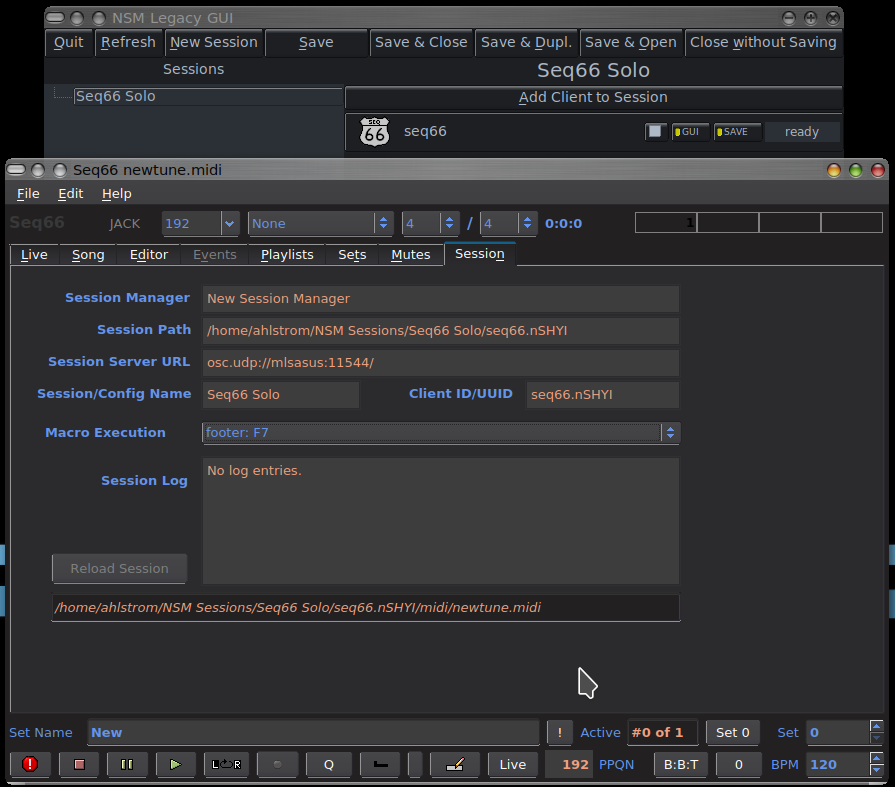
\includegraphics[scale=0.65]{tabs/session/qseq66-session-tab.png}
   \caption*{Session Tab When Running Under NSM}
\end{figure}

   Note: this diagram is a bit out of date.  Missing are the status of the
   controls, which are disabled, as most are for information only.
   Also missing are the \textbf{Reload Session} button and the
   \textbf{Macro Execution} drop-down, which are described below.

   \index{sessions!ui}
   This section describes the \textsl{Session} tab in the main
   \textsl{Seq66} window.  This tab is merely informative and
   \textsl{read-only}.
   It displays the following bits of information that \textsl{Seq66} has received
   from \textsl{NSM} via the \texttt{nmsd} daemon:

   \begin{itemize}
      \item Name of the session manager.
      \item Session path for the session, the root directory of the session.
         All data goes into this directory. If not running in a session,
         the active configuration directory (which can be modified via
         command-line arguments) is shown.
      \item The OSC URL of the session, which includes the port number.
         Generally, the port number is selected at run-time, but it is also
         possible to configure \textsl{NSM} to use a specific port number.
      \item Display-name for the session.
      \item The generated client ID for the session.
      \item The log of action of the session manager. Not yet supported,
         though one can see what is happening by running in a console window.
      \item Macro Execution.
         This drop-down contains all of the macros defined in the 'ctrl' file's
         \texttt{[macro-control-out]} section.
         By selecting one, it is automatically sent out via the
         \texttt{[output-buss]} port defined in the 'ctrl' file.
      \item Reload Session.
         After editing some of the preferences in the \textbf{Edit / Preferences}
         dialog, one can visit this tab and press this button to essentially
         restart \textsl{Seq66}, reloading the new configuration.
         Be careful!
   \end{itemize}

\subsubsection{Seq66 Session Management / NSM / File Menu}
\label{subsubsec:sessions_file_menu}

   The author of \textsl{NSM} has provided documentation for session-management
   which provides very strict instructions on how an application must behave
   under session management.  \textsl{Seq66} tries very hard to stick to these
   instructions.  One major adjustment an application must make is to adhere to
   the "File menu" guidelines.

\begin{figure}[H]
   \centering 
   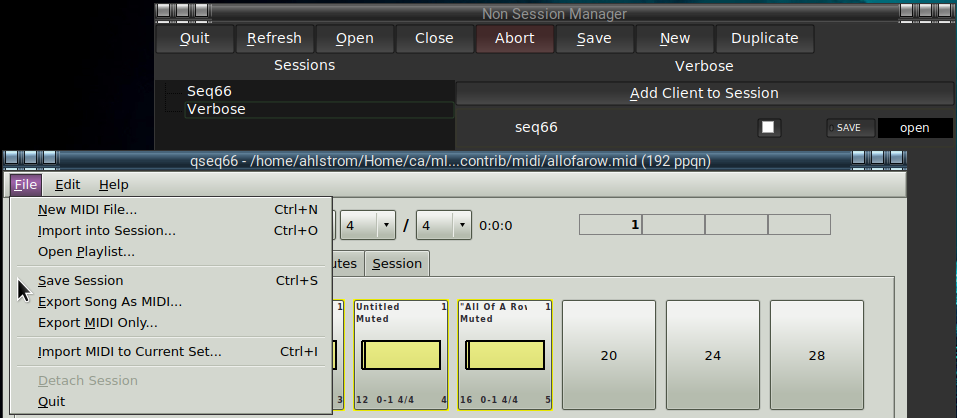
\includegraphics[scale=0.65]{tabs/session/nsm-qseq66-menus.png}
   \caption*{File Menu When Running Under NSM}
\end{figure}

   The following items describe the menu entries.

   \begin{itemize}
      \item \textbf{New MIDI File}.
         This function prompts for the name of a
         new MIDI file and clears the current MIDI file.  The file-name must not
         include a full-path to the file.  The path is hardwired by the
         session.  A relative path can be included.  This name is needed
         because there is no "Save As" option when running in an \textsl{NSM}
         session.
      \item \textbf{Import into Session}.
         Prompts the user for a MIDI file to
         be imported (copied) into the current session.  The path to the file
         is then adjusted to use the \textsl{NSM} \texttt{midi} subdirectory.
      \item \textbf{Open Playlist}.
         Works the same as without session
         management, but gets the list from the session directory.
      \item \textbf{Save Session}.
         This function saves the main configuration
         files (except for the 'usr' file), saves the play-list and note-mapper
         files, if in use, and saves the current MIDI file, if any.
      \item \textbf{Export Song As MIDI}.
         Allows exporting the current song as a stock MIDI file, using the
         performance information (triggers) to write the MIDI data as it would
         be played in "song" mode.
         The default directory that comes up in the
         prompt is the "last-used directory" from the session 'rc' file.
      \item \textbf{Export MIDI Only}.
         Allows exporting the current song as a stock MIDI file.
         The "proprietary" SeqSpec data is \textsl{not} written.
         The default directory that comes up in the
         prompt is the "last-used directory" from the session 'rc' file.
      \item \textbf{Import MIDI to Current Set}.
         This item allows the user to grab a MIDI file from anywhere and import
         it into the current set.
         The default directory that comes up in the
         prompt is the "last-used directory" from the session 'rc' file.
      \item \textbf{Detach}.
         Allows \textsl{Seq66} to detach from session management.
         This process simply disconnects from \textsl{NSM} and restores the
         normal \textsl{File} menu.
         Currently, it is disabled because it causes issues that we cannot yet
         solve.
      \item \textbf{Quit}.
         Quits \textsl{Seq66}.
         There are no messages to send to \textsl{NSM} in this case.
         The \texttt{nsmd} daemon detects that the \textsl{Seq66} client has
         disappeared (and notes that on the console output, if available).
   \end{itemize}

   At some point we would like to present a small tutorial showing a session
   under \textsl{JACK}.

   Also note that NSM can invoke or kill applications via
   \textsl{signals}, as explained in 
   \sectionref{subsec:sessions_signals}.

\subsubsection{Seq66 Session Management / NSM / Debugging}
\label{subsubsec:sessions_debugging}

   This section is oriented towards advanced users who found a problem running
   \textsl{Seq66} and want to track it down themselves.  The issue is that we
   need to start the application under the debugger, or start it under NSM and
   somehow attach to \textsl{Seq66} before it starts running.  Another issue is
   that we have found that, at least on the same host, an NSM session
   \textsl{must} be open before \textsl{Seq66} can attach to it, even if the
   correct \texttt{NSM\_URL} is provided.
   So we have to open a session, get the proper URL, configure it in the 'usr'
   file, and then start \textsl{Seq66} under the debugger.
   Here are the steps:

   \begin{enumerate}
      \item Start \textsl{non-session-manager} from a command-line console.
         Write down the URL that it advertises.
      \item Prepare a session for the executable as per earlier instructions.
         Once \texttt{qseq66} starts, immediately exit it, and leave the session
         open.
      \item Open the proper 'usr' file (usually \texttt{qseq66.usr}) in a 
         text editor.  Set variable "session = nsm", and set the variable "url"
         to the value that was advertised.
      \item Now start \texttt{qseq66} in a debugger.
      \item Set a breakpoint in \texttt{clinsmanager::detect\_session()}.
   \end{enumerate}
   
   Now you can step through and see where NSM and Seq66 are getting mixed up.
   Also check the session directory afterward to make the configuration
   (and any MIDI files) are in good shape.

\subsection{Seq66 Session Management / LASH}
\label{subsec:sessions_lash}

   \index{sessions!lash}
   LASH support has been removed.  Use the \textsl{NSM Session Manager} or
   the \textsl{JACK Session Manager}.

%-------------------------------------------------------------------------------
% vim: ts=3 sw=3 et ft=tex
%-------------------------------------------------------------------------------
